\documentclass[11pt]{article}
\usepackage[utf8]{inputenc}
\usepackage[affil-it]{authblk}
\usepackage{amsmath}
\usepackage{fullpage}
\usepackage{hyperref}
\usepackage{tikz}
\usepackage{calc}
\usepackage{pgfplots}
\usepackage{float}
\usepackage{caption}
\usetikzlibrary{automata}
\title{\textbf{Hidden Markov Model Cheatsheet}}
\author{Kanru Hua%
  \thanks{Email address: \texttt{khua5@illinois.edu}}}
\affil{University of Illinois at Urbana-Champaign}
\date{April 2016}
\begin{document}

\maketitle

\section{Preliminaries}

\begin{align*}
\intertext{\textbf{Conditional (Posterior) Probability}}
P(A|B) &= \frac{P(A, B)}{P(B)}
\intertext{where $P(A, B)$ is called \textbf{joint probability} and $P(B)$ is called \textbf{prior probability}.}
\intertext{\textbf{Statistical Independence}}
\intertext{If A and B are independent events,}
P(A|B) = P(A) &\textrm{\ and\ } P(B|A) = P(B) \\
\textrm{or\ } P(A, B) &= P(A) P(B)
\intertext{\textbf{Marginal Probability}}
P(A) &= \sum_b P(A, B = b)
\intertext{\textbf{Expectation}}
E[X] &= \sum_j P(X = x_j) x_j
\intertext{\textbf{Jensen's Inequality}}
\intertext{(You are \textbf{not} required to know this beforehand)}
E[f(X)] &\leq f(E[X]) \textrm{\ for any concave function $f$} \\
E[f(X)] &= f(E[X]) \textrm{\ if X is constant}
\end{align*}

\section{Markov Chain}

\subsection{Example}

\newcommand{\placeholder}[1]{\phantom{aaa}\makebox[0pt]{#1}\phantom{aaa}}
\begin{center}
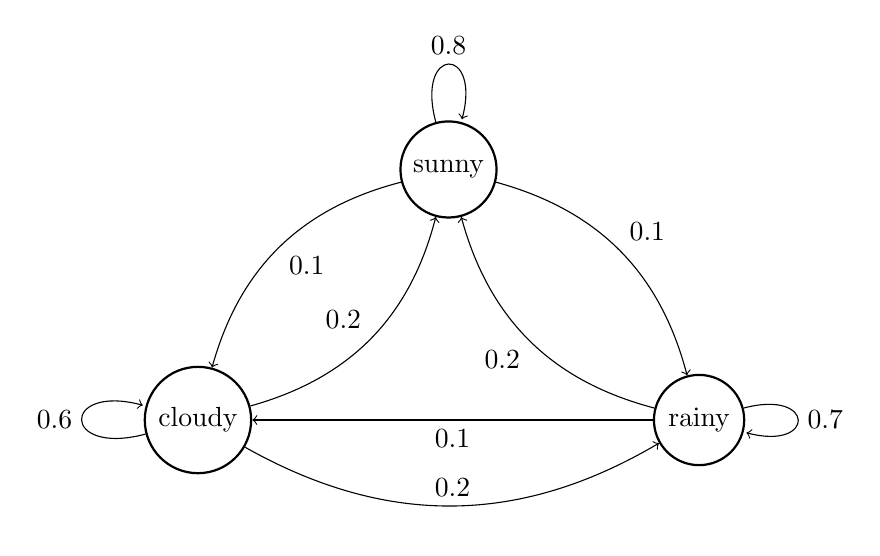
\begin{tikzpicture}[->,auto,node distance=4.5cm]
\tikzstyle{every state}=[fill=white,draw=black,thick,text=black,scale=1]
\node[state]    (A)                     {\placeholder{sunny}};
\node[state]    (B)[below left of=A]    {\placeholder{cloudy}};
\node[state]    (C)[below right of=A]   {\placeholder{rainy}};
\path (A) edge[loop above]     node{0.8}         (A);
\path (A) edge[bend right]     node{0.1}         (B);
\path (A) edge[bend left]      node{0.1}         (C);
\path (B) edge[loop left]      node{0.6}         (B);
\path (B) edge[bend right]     node{0.2}         (A);
\path (B) edge[bend right]     node{0.2}         (C);
\path (C) edge[loop right]     node{0.7}         (C);
\path (C) edge[bend left]      node{0.2}         (A);
\path (C) edge     			   node{0.1}         (B);
\end{tikzpicture}
\end{center}

\subsection{Definition}

\begin{align*}
\textrm{parameter set:\quad} &\lambda = \{\pi, \mathbf{A}\} \\
\textrm{initial probability:\quad}&\pi_j = P(s_1 = j | \lambda) \\
\textrm{transition probability:\quad}&a_{ij} = P(s_t = j | s_{t-1} = i, \lambda)
\intertext{\textbf{Markov Property}}
P(s_t = j | s_1, s_2, ..., s_{t-2}, s_{t-1} = i, \lambda) &= P(s_t = j | s_{t-1} = i, \lambda) = a_{ij}
\end{align*}

A lateral view where each edge has a transition probability, or an initial probability for $t = 1$:
\begin{center}
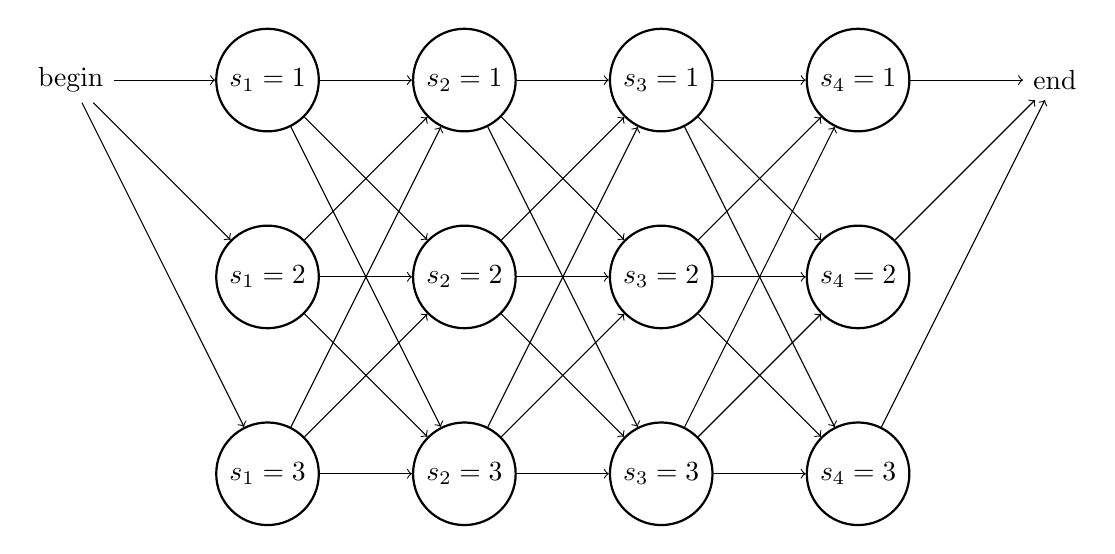
\begin{tikzpicture}[->,auto,node distance=2.5cm]
\tikzstyle{every state}=[fill=white,draw=black,thick,text=black,scale=1]
\tikzstyle{ends}=[fill=white,draw=white,thick,text=black,scale=1]
\node[ends]     (0)                {begin};
\node[state]    (A)[right of=0]    {\placeholder{$s_1=1$}};
\node[state]    (B)[right of=A]    {\placeholder{$s_2=1$}};
\node[state]    (C)[right of=B]    {\placeholder{$s_3=1$}};
\node[state]    (D)[right of=C]    {\placeholder{$s_4=1$}};
\node[state]    (A1)[below of=A]   {\placeholder{$s_1=2$}};
\node[state]    (B1)[right of=A1]  {\placeholder{$s_2=2$}};
\node[state]    (C1)[right of=B1]  {\placeholder{$s_3=2$}};
\node[state]    (D1)[right of=C1]  {\placeholder{$s_4=2$}};
\node[state]    (A2)[below of=A1]  {\placeholder{$s_1=3$}};
\node[state]    (B2)[right of=A2]  {\placeholder{$s_2=3$}};
\node[state]    (C2)[right of=B2]  {\placeholder{$s_3=3$}};
\node[state]    (D2)[right of=C2]  {\placeholder{$s_4=3$}};
\node[ends]     (1)[right of=D]    {end};
\path (0) edge (A);\path (0) edge (A1);\path (0) edge (A2);
\path (A) edge (B);\path (A) edge (B1);\path (A) edge (B2);
\path (B) edge (C);\path (B) edge (C1);\path (B) edge (C2);
\path (C) edge (D);\path (C) edge (D1);\path (C) edge (D2);
\path (D) edge (1);\path (D1) edge (1);\path (D2) edge (1);
\path (A1) edge (B1);\path (A1) edge (B);\path (A1) edge (B2);
\path (B1) edge (C1);\path (B1) edge (C);\path (B1) edge (C2);
\path (C1) edge (D1);\path (C1) edge (D);\path (C1) edge (D2);
\path (A2) edge (B2);\path (A2) edge (B);\path (A2) edge (B1);
\path (B2) edge (C2);\path (B2) edge (C);\path (B2) edge (C1);
\path (C2) edge (D2);\path (C2) edge (D);\path (C2) edge (D1);
\end{tikzpicture}
\end{center}

\section{Hidden Markov Model}

\subsection{Definition}

\begin{align*}
\textrm{parameter set:\quad} &\lambda = \{\pi, \mathbf{A}, \mathbf{B}\} \\
\textrm{initial probability:\quad}&\pi_j = P(s_1 = j | \lambda) \\
\textrm{transition probability:\quad}&a_{ij} = P(s_t = j | s_{t-1} = i, \lambda) \\\\
\textrm{output probability (discrete case):\quad}&b_{jk} = P(o_t = k | s_t = j, \lambda) \\
\textrm{output probability density (continuous case):\quad}&b_j(o_t) = p(o_t | s_t = j, \lambda)
\end{align*}

\subsection{Graph}
\begin{center}
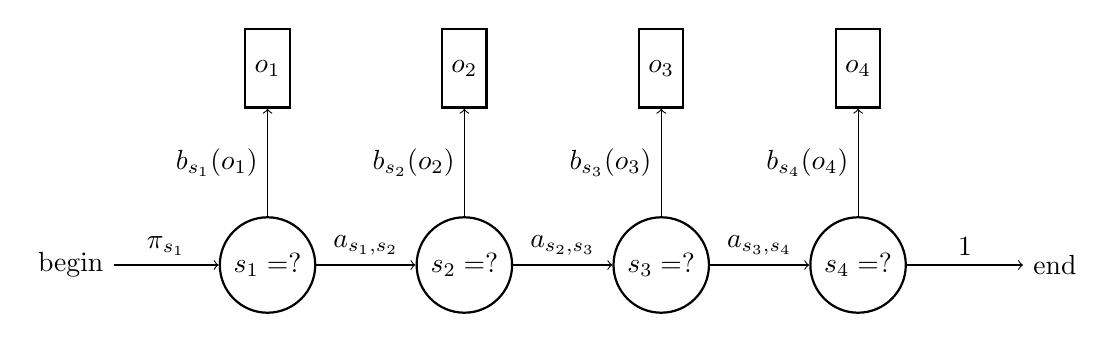
\begin{tikzpicture}[->,auto,node distance=2.5cm]
\tikzstyle{every state}=[fill=white,draw=black,thick,text=black,scale=1]
\tikzstyle{output}=[fill=white,draw=black,thick,text=black,scale=1,minimum height=1cm]
\tikzstyle{ends}=[fill=white,draw=white,thick,text=black,scale=1]
\node[ends]     (0)                {begin};
\node[state]    (A)[right of=0]    {\placeholder{$s_1=?$}};
\node[state]    (B)[right of=A]    {\placeholder{$s_2=?$}};
\node[state]    (C)[right of=B]    {\placeholder{$s_3=?$}};
\node[state]    (D)[right of=C]    {\placeholder{$s_4=?$}};
\node[output]   (Ao)[above of=A]   {\placeholder{$o_1$}};
\node[output]   (Bo)[above of=B]   {\placeholder{$o_2$}};
\node[output]   (Co)[above of=C]   {\placeholder{$o_3$}};
\node[output]   (Do)[above of=D]   {\placeholder{$o_4$}};
\node[ends]     (1)[right of=D]    {end};
\path (0) edge node{$\pi_{s_1}$}   (A);
\path (A) edge node{$a_{s_1,s_2}$} (B);
\path (B) edge node{$a_{s_2,s_3}$} (C);
\path (C) edge node{$a_{s_3,s_4}$} (D);
\path (D) edge node{$1$}           (1);
\path (A) edge node{$b_{s_1}(o_1)$}(Ao);
\path (B) edge node{$b_{s_2}(o_2)$}(Bo);
\path (C) edge node{$b_{s_3}(o_3)$}(Co);
\path (D) edge node{$b_{s_4}(o_4)$}(Do);
\end{tikzpicture}
\end{center}

\subsection{List of Operations \& Algorithms}

What can we do with HMM?

\begin{itemize}
\item Generation
  \begin{itemize}
    \item Random walk
  \end{itemize}
\item Inference
  \begin{itemize}
    \item \textbf{Forward/Backward algorithm}
    \item \textbf{Viterbi algorithm}
    \item Total probability: $P(O | \lambda)$
    \item State occupancy probability: $P(s_t = j | O, \lambda)$
    \item Optimal probability \& state sequence: $\underset{s}{\arg\max\\ } P(O, s | \lambda)$
  \end{itemize}
\item Parameter estimation (training)
  \begin{itemize}
    \item Initialization
    \item Viterbi training
    \item \textbf{Baum-Welch algorithm} (expectation-maximization)
  \end{itemize}
\end{itemize}

\newpage
\section{HMM Inference}

\subsection{Building Blocks}

\begin{align*}
\intertext{What we already know:}
P(s_1 = i | \lambda) &= \pi_i \\
P(s_t = j | s_{t - 1} = i, \lambda) &= a_{ij} \\
P(o_t | s_t = j, \lambda) &= b_j(o_t)
\intertext{Trivial extensions using Markov property:}
P(s_1, s_2, ..., s_t | \lambda) &= \pi_{s_1} \prod_{\tau=2}^t a_{\tau-1,\tau} \\
P(o_1, o_2, ..., o_t | s_1, s_2, ..., s_t, \lambda) &= \prod_{\tau=1}^t b_{s_\tau}(o_\tau)
\intertext{By combining above equations, we get}
P(o_1, o_2, ..., o_t, s_1, s_2, ..., s_t | \lambda) &= \pi_{s_1} b_{s_1}(o_1) \prod_{\tau=2}^t a_{\tau-1,\tau} b_{s_\tau}(o_\tau)
\end{align*}

\subsection{Inference Algorithms}

\begin{align*}
\intertext{\textbf{Forward Algorithm}}
\alpha_t(i) &= P(o_1, o_2, ..., o_t, s_t=i | \lambda) \\
            &= P(o_t | s_t=i, \lambda) \sum_j P(o_1, ..., o_{t-1}, s_{t-1}=j | \lambda) P(s_t=i | s_{t-1}=j, \lambda) \\
            &= b_i(o_t) \sum_j a_{ji} \alpha_{t-1}(j) \\
\alpha_1(i) &= P(o_1 | s_1 = i, \lambda) P(s_1=i | \lambda) = b_i(o_1) \pi_i
\intertext{\textbf{Backward Algorithm}}
\beta_t(i)  &= P(o_{t+1}, o_{t+2}, ..., o_t | s_t=i, \lambda) \\
            &= \sum_j P(o_{t+1} | s_{t+1}=j, \lambda) P(o_{t+2}, ..., o_T | s_{t+1}=j, \lambda) P(s_{t+1}=j | s_t=i, \lambda) \\
            &= \sum_j b_j(o_{t+1}) \beta_{t+1}(j) a_{ij} \\
\beta_T(i)  &= 1
\intertext{\textbf{Viterbi Algorithm}}
\alpha^*_t(i)
            &= \max_{s_1, ..., s_{t-1}} P(o_1, ..., o_t, s_1, ..., s_{t-1}, s_t = i | \lambda) \\
            &= P(o_t | s_t=i, \lambda) \max_j \left( P(s_t=i | s_{t-1}=j, \lambda) \max_{s_1, ..., s_{t-2}} P(o_1, ..., o_{t-1}, s_1, ..., s_{t-2}, s_{t-1}=i | \lambda) \right) \\
            &= b_i(o_t) \max_j a_{ji} \alpha^*_{t-1}(j) \\
p^*_t(i)    &= \underset{j}{\arg\max\ } a_{ji} \alpha^*_{t-1}(j) \\
\alpha^*_1(i)
            &= b_i(o_1) \pi_i \\
p^*_1(i)    &= 0
\intertext{\textbf{Total Probability}}
P(O | \lambda) &= \sum_j P(o_1, ..., o_T, s_t=j | \lambda) = \sum_j \alpha_T(j) \textrm{\quad (from forward probability)} \\
P(O | \lambda) &= \sum_j P(o_1 | s_1=j, \lambda) P(o_2, ..., o_T | s_1=j, \lambda) P(s_1=j | \lambda) \\
               &= \sum_j b_j(o_1) \beta_1(j) \pi_j \textrm{\quad (from backward probability)} \\
P(O | \lambda) &= \sum_j P(o_1, ..., o_t, o_{t+1}, ..., o_T, s_t=j | \lambda) \\
               &= \sum_j P(o_1, ..., o_t, s_t=j | \lambda) P(o_{t+1}, ..., o_T | s_t=j, \lambda) \\
               &= \sum_j \alpha_t(j) \beta_t(j) \textrm{\quad (from both forward and backward probability, for arbitrary $t$)}
\intertext{\textbf{State Occupancy Probability}}
\gamma_t(j) &= P(s_t=j | O, \lambda) \\
            &= \frac{P(o_1, ..., o_t, s_t=j | \lambda) P(o_{t+1}, ..., o_T | s_t=j, \lambda)}{P(O | \lambda)} \\
            &= \frac{\alpha_t(j) \beta_t(j)}{P(O | \lambda)}
\intertext{note that $\sum_j \gamma_t(j) = 1$}
\intertext{\textbf{State Transition Probability} (not to be confused with $a_{ij}$)}
\gamma_t(i, j) &= P(s_{t-1}=i, s_t=j | O, \lambda) \\
               &= \frac{\alpha_{t-1}(i) \beta_t(j) b_j(o_t) a_{ij}}{P(O | \lambda)} \quad\textrm{whose derivation is similar to $\gamma_t(j)$}
\end{align*}

\newpage
\section{HMM Parameter Estimation}

\subsection{Expectation-Maximization Algorithm}

\begin{align*}
\intertext{Goal: obtain maximum likelihood estimation of $\lambda$:}
\lambda^* &= \underset{\lambda}{\arg\max\ } l(\lambda) = \underset{\lambda}{\arg\max\ } \log P(O | \lambda) \\
l(\lambda) &= \log P(O | \lambda) = \log \sum_\mathbf{s} P(O, \mathbf{s} | \lambda)
\intertext{Motivation: find an alternative likelihood function whose derivatives are easier to calculate.}
\intertext{Assume we have a function $Q(\mathbf{s})$ such that $\sum_\mathbf{s} Q(\mathbf{s}) = 1$ and $Q(\mathbf{s}) > 0 \ \forall \mathbf{s}$,}
l(\lambda) &= \log \sum_\mathbf{s} Q(\mathbf{s}) \frac{P(O, \mathbf{s} | \lambda)}{Q(\mathbf{s})} \\
  &= \log E_{\mathbf{s}} [\frac{P(O, \mathbf{s} | \lambda)}{Q(\mathbf{s})}] \\
  &\geq E_{\mathbf{s}} [\log \frac{P(O, \mathbf{s} | \lambda)}{Q(\mathbf{s})}] \quad\textrm{(whose partial derivatives have closed form)}
\intertext{To make the lower bound more ``effective", i.e., we want $\log E_s [...] = E_s [\log (...)]$,}
&\begin{cases}
  \frac{P(O, \mathbf{s} | \lambda}{Q(\mathbf{s})} &= c \\
  \sum_\mathbf{s} Q(\mathbf{s}) &= 1
\end{cases} \ \Rightarrow Q(\mathbf{s}) = P(\mathbf{s} | O, \lambda)
\end{align*}

\subsubsection*{EM Algorithm}

\noindent
Repeat until convergence \{

Expectation: $Q(\mathbf{s}) = P(\mathbf{s} | O, \lambda)$

Maximization: $\lambda^* = \underset{\lambda}{\arg\max\ } \sum_\mathbf{s} Q(\mathbf{s}) \log \frac{P(O, \mathbf{s} | \lambda)}{Q(\mathbf{s})}$

\noindent
\}

\subsection{Baum-Welch Algorithm}

\begin{align*}
\intertext{Error function (in maximization step):}
J(\lambda) &= \sum_\mathbf{s} Q(\mathbf{s}) \log \frac{P(O, \mathbf{s} | \lambda)}{Q(\mathbf{s})} \\
  &= \sum_\mathbf{s} Q(\mathbf{s}) \left( \log \pi_{s_1} + \sum_{t=2}^T \log a_{s_{t-1},s_t} + \sum_{t=1}^T \log b_{s_t}(o_t) - \log(Q(\mathbf{s})) \right)
\intertext{Take partial derivative with respect to, for example, $a_{ij}$,}
\frac{\partial J}{\partial a_{ij}}
  &= \frac{\partial}{\partial a_{ij}} \sum_\mathbf{s} Q(\mathbf{s}) \sum_{t=2}^T \log a_{s_{t-1},s_t} \\
  &= \frac{\partial}{\partial a_{ij}} \sum_{t=2}^T \sum_m \sum_n \log a_{mn} \sum_\mathbf{\substack{s_1,..., s_{t-2} \\ s_{t+1}, ..., s_T}} Q(\mathbf{s}) \\
  &= \frac{\partial}{\partial a_{ij}} \sum_{t=2}^T \sum_m \sum_n \log a_{mn} \underbrace{P(s_{t-1}=m, s_t=n | O, \lambda')}_{\gamma_t(m, n)} \\
  &= \frac{1}{a_{ij}} \sum_{t=2}^T \gamma_t(i, j)
\intertext{To make sure $\sum_j a_{ij} = 1 \ \forall i$, introduce Lagrange multiplier $l$,}
&\begin{cases}
  \sum_{t=2}^T \gamma_t(i, j) &= l a_{ij} \\
  \sum_j a_{ij} &= 1
\end{cases}
\intertext{Solve the equations,}
l &= \sum_{t=2}^T \sum_n \gamma_t(i, n), \quad a_{ij} = \frac{\sum_{t=2}^T \gamma_t(i, j)}{\sum_{t=2}^T \sum_n \gamma_t(i, n)} = \frac{\sum_{t=2}^T \gamma_t(i, j)}{\sum_{t=2}^T \gamma_{t-1}(i)}
\intertext{Similarly for $\pi_i$ and $b_{ik}$ (discrete case) we get,}
\pi_i &= \gamma_1(i) \\
b_{ik} &= \frac{\sum_{t: o_t = k} \gamma_t(i)}{\sum_{t=1}^T \gamma_t(i)}
\intertext{\textbf{Multiple Observation Sequences}}
\pi_i &= \frac{1}{L} \sum_{l=0}^L \gamma_1^l(i) \\
a_{ij} &= \frac{\sum_{l=0}^L \sum_{t=2}^T \gamma_t^l(i, j)}{\sum_{l=0}^L \sum_{t=2}^T \gamma_{t-1}^l(i)}
\quad b_{ik} = \frac{\sum_{l=0}^L \sum_{t: o_t = k} \gamma_t^l(i)}{\sum_{l=0}^L \sum_{t=1}^T \gamma_t^l(i)}
\end{align*}

\subsection{Baum-Welch Algorithm for Continuous Output Distributions}

\begin{alignat*}{3}
\intertext{\textbf{Multivariate Normal Distribution}}
\mu_j &= \frac{\sum_{t=1}^T \gamma_t(j) o_t}{\sum_{t=1}^T \gamma_t(j)} \quad &\Sigma_j &= \frac{\sum_{t=1}^T \gamma_t(j) o_t o_t^T}{\sum_{t=1}^T \gamma_t(j)} - \mu_j \mu_j^T
\end{alignat*}
\begin{align*}
\intertext{\textbf{Multivariate Gaussian Mixture Model}}
\intertext{Gaussian mixture model:}
p(x \in \mathbf{R}^k | \boldsymbol c, \boldsymbol\mu, \boldsymbol\Sigma) &= (2\pi)^{-\frac{k}{2}} \sum_j c_j |\Sigma_j|^{-\frac{k}{2}} e^{-\frac{k}{2} (x - \mu_j)^T \Sigma_j^{-1} (x - \mu_j)}
\intertext{HMM-GMM:}
g_{jk}(o_t) &= p(o_t | s_t=j, m_t = k, \lambda) = p(o_t | \boldsymbol \mu_{jk}, \boldsymbol \Sigma_{jk}) \\
b_j(o_t) &= p(o_t | s_t=j, \lambda) = \sum_k c_{jk} g_{jk}(o_t)
\intertext{HMM-GMM inference:}
\xi_t(j, k) &= p(s_t=j, m_t=k | O, \lambda) = \frac{\sum_i \alpha_{t-1}(i) \beta_t(j) a_{ij}c_{jk}g_{jk}(o_t)}{P(O | \lambda)}
\end{align*}
\begin{alignat*}{3}
\intertext{HMM-GMM parameter estimation:}
c_{jk} &= \frac{\sum_{t=1}^T \xi_t(j, k)}{\sum_{t=1}^T \gamma_t(j)} \\
\mu_{jk} &= \frac{\sum_{t=1}^T \xi_t(j, k) o_t}{\sum_{t=1}^T \xi_t(j, k)} \quad &\Sigma_{jk} &= \frac{\sum_{t=1}^T \xi_t(j, k) o_t o_t^T}{\sum_{t=1}^T \xi_t(j, k)} - \mu_{jk} \mu_{jk}^T
\end{alignat*}

\begin{thebibliography}{99}

\bibitem{mmprta}{Fink, Gernot A. ``Markov models for pattern recognition: from theory to applications". Springer Science \& Business Media, 2014.}

\bibitem{cs229}{Ng, Andrew. ``Mixtures of Gaussians and the EM algorithm." Stanford University. CS229 Lecture Notes (2014).}

\bibitem{bilmes}{Bilmes, Jeff A. ``A gentle tutorial of the EM algorithm and its application to parameter estimation for Gaussian mixture and hidden Markov models." International Computer Science Institute 4.510 (1998): 126.}

\end{thebibliography}

\end{document}
